
The Bluetooth stack has many layers. For this project the important layers are the HCI, LMP, and the physical layer(Bluetooth Radio). As seen in figure \ref{fig:bt_stack}. The LMP have already been discussed in an earlier section. The HCI and the physical layer will be discussed below.

\begin{figure}[h]
  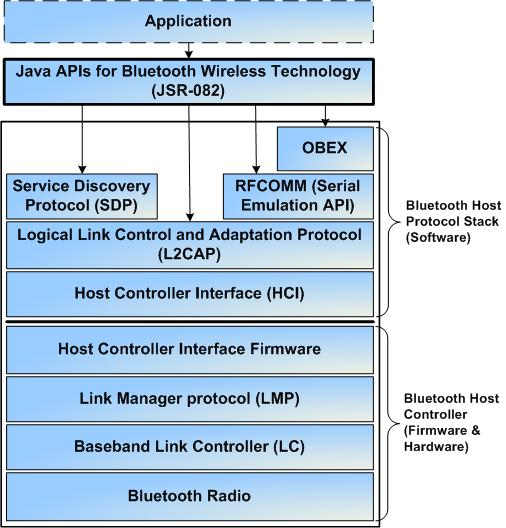
\includegraphics[scale=0.8]{images/bluetoothstack.jpg}
  \caption{The Bluetooth stack}
  \label{fig:bt_stack}
  \captionsetup{font={footnotesize,bf,it}}
  \caption*{\url{http://www.oracle.com/technetwork/testcontent/fig1-1-158000.jpg}}
\end{figure}
\newpage
\subsubsection{Physical layer}
	% How we Gather data form the ubertooth
	In order to eavesdrop a Bluetooth communication, the Ubertooth One presented above has been used. This tool is able to decode packet from a targeted Bluetooth communication. \pend
	The LAP was known for the two devices. As explained in the literature review, the Ubertooth tool retrieve the important parameters (UAP, clocks) used to sniff a connection thanks to that address. Once the tool was able to sniff and follow the
	 communication between the two devices it was possible for it to decode packets.
	In order to have relevant information the authors conducted experiments in a certain way. Indeed several captures have been performed recording:
\begin{itemize}
	\item[•] The pairing process between the two devices
	\item[•] The de-authentication process between two devices
	\item[•] The exchange of different data format (videos, pictures, notification) 
\end{itemize}
		 
\subsubsection{HCI layer}
	% How we Gather data form the hci
Due to the increasing use of Bluetooth; Android, since Android 4.4, has added a functionality for developers to sniff Bluetooth packets at the HCI layer. This tool allows to monitor Bluetooth traffic in forms of pcaps logs for Wireshark. These logs can be found in the root of your data directory and is called btsnoop\_hci\.log.\pend
The HCI layer is just above the LMP layer where authentication and encryption/encapsulation takes place. This can be seen in figure \ref{fig:bt_stack}. The data and messages exchanged at this layer are in clear text and packets are not encapsulated. This makes them easily identifiable and easy to monitor. \pend
The experiments performed above at the Physical layer has been performed in the same way (and at the same time) at the HCI layer. Both tools need to be run at the same time to compare the data.
	